\documentclass[12pt]{article}
\usepackage[a4paper, margin=.30in]{geometry}
\usepackage{graphicx ,
            wrapfig,
            xcolor, 
            enumerate,
            amsmath,fontenc,makecell,chemfig, multirow
            }

\newcommand\headerMe[2]{\noindent{}#1\hfill#2}
\renewcommand{\thesection}{\Roman{section}}

%\title{Leçon N 6 : Le mouvement}
\author{Zakaria HAOUZAN}
\date{\today}

\begin{document}
% headers --------------
\headerMe{Matière : Physique-Chimie}{Professeur : Zakaria HAOUZAN}\\
\headerMe{Unité : Travail Mécanique et Energie }{Établissement : Lycée SKHOR qualifiant}\\
\headerMe{Niveau : TCS}{Heure : 4H}\\

% ------Content ________
\begin{center}

    \Large{Leçon $N^{\circ} 4 $: \color{red} La quantité de matière : la mole}
\end{center}

%\begin{wrapfigure}[10]{r}{0.5\textwidth}
%    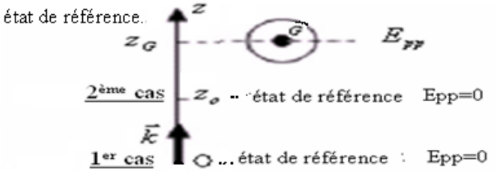
\includegraphics[width=0.5\textwidth]{./img/img00.png}
%\end{wrapfigure}

\section{Notion de mole: }
\subsection{Définition: }
La quantité de matière d'un échantillon est le nombre de moles que contient cet échantillon, c'est une grandeur
notée n ; son unité est la mole (mol).

Une mole de particules (atomes, molécules etc) est définie comme un ensemble de $6,02.10^{23}$ particules identiques .

Le nombre de particules contenues dans une mole s'appelle le nombre d'Avogadro: $N_A = 6,02.10^{23}mol^{-1}$

Relation entre la quantité de matière et le nombre d'Avogadro: La quantité de matière n d'un échantillon qui contient N particules identiques est donnée par la relation suivante : $n = \frac{N}{N_A}$

\section{Masse molaire atomique et masse molaire moléculaire:}
\subsection{Masse molaire atomique :}
La masse molaire atomique d’un élément chimique X est la masse d’une mole d’atomes de cet élément. (unité g/mol)

Le symbole de la masse atomique d’un élément chimique X est M(X).
Exemples : On donne la masse des atomes des éléments suivants:
\\H : $m(H) = 0.167.10^{-26}Kg$
\\C : $m(C) = 1.993.10^{-26}Kg$
\\O : $m(O) = 2.658.10^{-26}Kg$

Déterminer la masse molaire atomique de chacun de ces éléments :
\\H : $ M(H)= N_A.m(H) =6.02x10^{23} . 0.167x10^{-26}Kg = 1g/mol$
\\C : $ M(C)= N_A.m(C) =6.02x10^{23} . 1.993x10^{-26}Kg = 12g/mol$
\\O : $ M(O)= N_A.m(O) =6.02x10^{23} . 2.658x10^{-26}Kg = 16g/mol$
\\N : $M(N) =14g/mol $
\\S : $M(N) =32g/mol $
\subsection{Masse molaire moléculaire: }
La masse molaire moléculaire d'une molécule est la somme des masses molaires atomiques des atomes qui
constituent cette molécule. (unité : g/mol)

Exemple: Déterminer les masses molaires moléculaires des molécules suivantes : $CH_4 . NH_3 , H_2SO_4 , H_2O$ 

\subsection{Relation entre la masse et la quantité de matière: }
La quantité de matière contenue dans une masse m(X) d'un corps constitué d'un élément chimique X est donnée par
la relation suivante: $n = \frac{m(X)}{M(X)}$
\\m(X) : masse du corps en g
\\M(X) : masse molaire du corps en (g/mol)
\\n(X) : quantité de matière en (mol)

Remarque : On a $m = \rho.V $ donc la quantité de matière: $n = \frac{\rho.V}{M}$

Exemple: Déterminer la quantité de matière contenue dans une masse m=3g de carbone .
On donne la masse atomique du carbone M(C) =12g/mol.

\section{Relation entre la quantité de matière et le volume molaire:}
\subsection{Le volume molaire des gaz:}
Le volume molaire d'un gaz $( V_M )$ : est le volume occupé par une mole de n'importe quel gaz pris dans des
conditions définies de température et de pression.

Remarque: Dans les conditions normales de température et de pression (P=1 atm et T = 0°C) : $V_M=22,4L/mol$.

\subsection{Volume et quantité de matière:}
La quantité de matière contenue dans un volume V d'un gaz est donnée par la relation suivante:$n = \frac{V}{V_m}$
\\n(X) : quantité de matière en (mol)
\\V    : volume de gaz  (L)
\\$V_M$: volume molaire   (L/mol)

Remarque: Pour les liquides et les solides , la densité est donnée par la relation suivante: $d = \frac{\rho}{\rho_{eau}}$ 
\\$\rho$: masse volumique du corps 
\\$\rho_{eau}$ : masse volumique de l'eau .
\\la quantité de matière $n = \frac{m}{M} = \frac{\rho.V}{M} = \frac{\rho_{eau}.d.V}{M}$
\subsection{Densité d'un gaz par rapport à l'air : }
\subsubsection{Définition:}
La densité d'un gaz est définie comme étant le rapport entre la masse d'un volume de gaz et la masse du même volume d’air. $$d = \frac{m_{gaz}}{m_{air}}$$ la densité est un nombre sans unité.
\subsubsection{Relation entre densité et masse molaire: }
Lorsqu'on s'interessse à une seule mole du gaz : V $->V_M$ et $m_{gaz}->M_{gaz}$ donc la relation précédente devient $$d = \frac{M_{gaz}}{M_{air}} = \frac{M_{gaz}}{\rho_{air}.V_M} = \frac{M_{gaz}}{1.293x22.4} = \frac{M_{gaz}}{29}$$

La densité d'un gaz par rapport à l'air est donc donnée par la relation : $$d = \frac{M_{gaz}}{29} $$
Mgaz: masse molaire du gaz.
Si $d>1$ le gaz est plus dense que l'air et si
$d<1$ le gaz est moins dense que l'air
\section{Equation d'état d'un gaz parfait:}
\subsection{Définition :}
On appelle gaz parfait un gaz dans lequel sont absentes les forces d'interactions .

À faibles pressions, où les interactions entre les molécules constitutives du gaz sont très faibles un gaz peut etre
assimilé à un gaz parfait.
\subsection{Loi des gaz parfaits: }
La loi des gaz parfaits est définie par la relation : $PV = nRT$
\\- P la pression en pascal.
\\- V le volume en $m^3$.
\\- T la température en °K.
\\- R la constante des gaz parfait en $J.mol^{-1}.K^{-1}$ . $R=8.314 en J.mol^{-1}.K^{-1}$
\end{document}

